%\chapter*{Введение}
%\addcontentsline{toc}{chapter}{Введение}

\newpage
\textbf {1 Медико-биологическая часть}
\refstepcounter{chapter}
\addcontentsline{toc}{chapter}{1 Медико-биологическая часть}

\section{Аналитический обзор мирового рынка медицинской робототехники}
Во всем мире, по данным The Robot Report \cite{litlink1}, существует более 343 компаний, производящих промышленных роботов, более 347 компаний, занимающихся интеграцией робототехнических комплексов в производственный процесс, более 886 компаний, производящих сервисных роботов для профессионального использования, и 204 компании, производящих сервисных роботов для персонального использования. На рисунке 1.1 видно, что наиболее перспективными областями развития робототехники являются транспорт и медицина.

\begin{figure}[!h]
\begin{center}
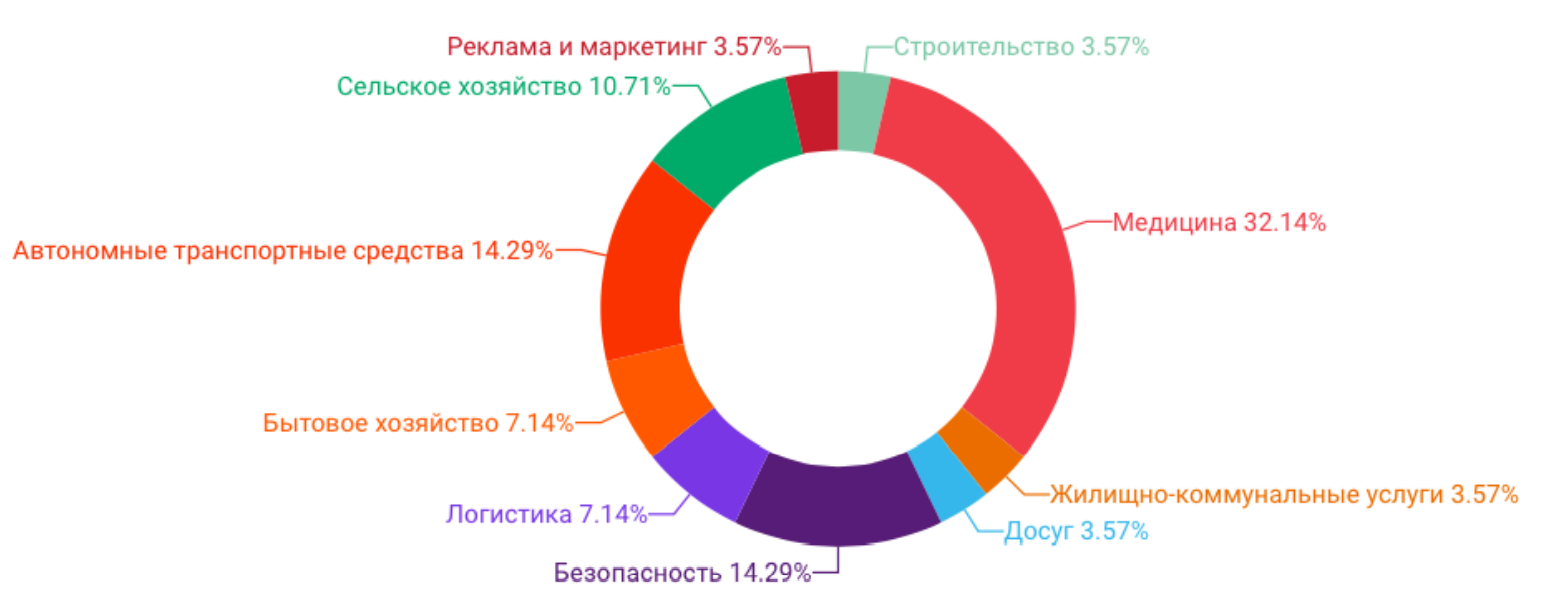
\includegraphics[width=0.9\textwidth]{Рисунки/диаграмма стата.png}
\caption{\centering \onehalfspacing {Перспективные области сервисной робототехники \cite{litlink2}}}
\label{част}
\end{center}
\end{figure}

Общий объем импорта роботизированных систем для медицинской диагностики в 2018 году составил 23,78 млн. долларов (в натуральном выражении – 16 шт.) \cite{litlink2}. Основными причинами внедрения медицинских роботизированных систем являются нехватка квалифицированного медперсонала, растущие заработные платы, рост потребности в автоматизации рутинных и монотонных процессов.Наиболее значительным фактором, способствующим росту рынка, являются общие экономические и социальные преимущества медицинской робототехники \cite{litlink3}. Кроме того, медицинская робототехника подходит для использования в гибридных операционных - одной из быстрорастущих технологий в медицинском секторе. Сдерживающий фактор - высокая стоимость закупки интегрированных роботизированных медицинских решений.

Наибольшие прибыли сконцентрированы в сегменте ассистивных хирургических комплексов (более 55\% от общего дохода мирового рынка). Наиболее популярные системы - Da Vinci и Teletap ALF-X. Используются машины для нейрохирургии, ортопедических процедур, некатетерных чрескожных и лапароскопических вмешательств, а также для управления роботизированными катетерами. Поскольку объем этих процедур велик во всем мире, предполагается, что этот сегмент сохранит свое доминирующее положение на рынке. По тепловой карте тематик публикаций в области медицинской робототехники (рисунок 1.2) можно заметить, что наиболее востребованы хирургические роботизированные системы.

\begin{figure}[!h]
\begin{center}
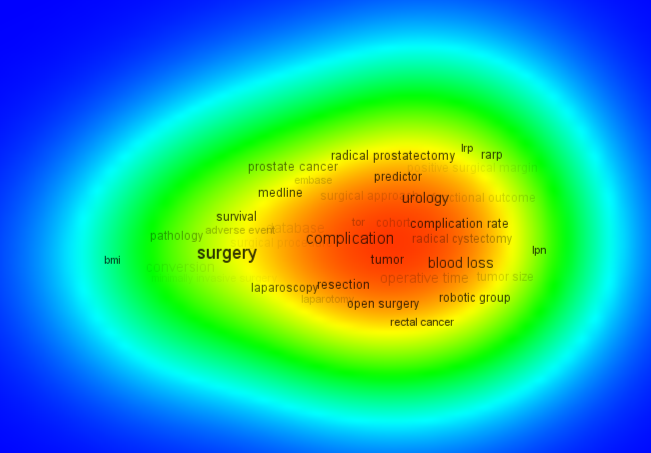
\includegraphics[width=0.7\textwidth]{Рисунки/тепловая карта.png}
\caption{\centering \onehalfspacing {Тепловая карта тематик публикаций кластера «Робототехника в медицине» \cite{litlink2}}}
\label{част}
\end{center}
\end{figure}

На ранних этапах развития возможности хирургических манипуляторов были крайне 
ограничены: не хватало вычислительных мощностей и пропускной способности каналов связи, а одной из ключевых проблем долгое время оставалась временная задержка между моментом отправки команд, производимым на операционном столе реальным хирургическим действием и итоговым получением визуального подтверждения этого действия на компьютерном мониторе. Однако рост вычислительных мощностей и пропускной способности каналов связи привели к тому, что в сентябре 2001 года была проведена первая телеуправляемая трансатлантическая операция. В этой операции использовалась первая универсальная роботизированная система Zeus, созданная в 1998 году, в состав которой входил усовершенствованный эндоскопический модуль AESOP \cite{litlink3}.

Рынок диагностического роботизированного оборудования также является крупнейшим сектором общего рынка медицинского оборудования \cite{litlink4}. Наиболее используемые роботы для медицинских систем, в том числе и для систем визуализации – коллаборативные роботы (коботы). Они состоят из манипулятора и устройства управления, в виде, например, планшета, которое формирует команды, задающие требуемые движения исполнительных органов манипулятора. В Abi Research сообщается  \cite{litlink4}, что среднегодовой прирост на рынке коботов в период с 2016 по 2025 год составит 50 \%.

Самые известные производители коллаборативных роботов — это компании Universal Robot, KUKA, Rethink Robotics и Franka. 

Медицинские роботы позволяют хирургам проводить операции более точным и менее инвазивным способом. Они используются из-за их способности выполнять повторяющиеся задачи на высоких скоростях без снижения качества из-за отсутствия фактора утомляемости. Роботизированный метод дает большие преимущества не только с точки зрения производительности, но и с точки зрения экономической эффективности. Основной целью внедрения медицинской робототехники является сокращение количество медицинских сотрудников и улучшение диагностических возможностей во время операции. 


%Существует телеультразвуковая система на базе робота французской компании AdEchoTech. Она обеспечивает возможность проводить ультразвуковое исследование под контролем обычного врача, когда эксперт в области УЗИ находится на удаленном расстоянии. В этой системе используется роботизированная рука Melody, позволяющая в реальном времени управлять удаленным от оператора датчиком и проводить диагностику.При этом система УЗИ-специалиста (Melody Expert) и система пациента (Melody Patient) работают совместно через Интернет и в реальном времени обмениваются информацией, а также обеспечивают управлением роботом. MELODY Patient очень точно повторяет движения, которые производит УЗИ-специалист. В ней используется имитатор зонда в виде копии стандартного ультразвукового датчика, с помощью которого можно контролировать движения робота издалека.Система сертифицирована FDA для использования на рынке США. И это единственная такая система.Вторая система имеет название HER (Hapticaly-Enabled Robotics) Remote Ultrasound, может применяться для исследования брюшной полости с целью оценки состояния почек, печени, желчного пузыря, поджелудочной железы, селезенки, а также брюшной аорты и других кровеносных сосудов. Система имеет встроенную технологию получения обратной связи от пациента, что позволяет специалисту дистанционно отслеживать дискомфорт пациента, связанный с силой давления УЗИ-датчика. Эта информация может использоваться для оценки чувствительности исследуемой области и для сравнения ее с данными предыдущих исследований пациента.Принципиальным преимуществом этой системы является ее способность транслировать чувство прикосновения оператора. Такая тактильная обратная связь помогает оператору ощущать удаленную среду посредством роботизированной системы. Для оценки ситуации, ощущения глубины восприятия и общения с пациентом используется система видеосвязи. Связь осуществляется посредство 4G-сети мобильной связи компании Telstra.Также аналогом является роботизированная система Tele Robotic Ultrasound for Distance или TRUDI, которая позволяет оператору проводить ультразвуковые исследования из любого места, где есть Интернет. Эта система интегрирована в роботизированный киоск, и оператор может ею управлять, манипулируя УЗИ-датчиком, легко устанавливая его в нужную позицию, что позволяет проводить исследование буквально за несколько минут.Система находится пока на ранней стадии разработки и когда она будет доведена до коммерческого уровня пока неизвестно.Для ее работы необходимо иметь телекоммуникационный канал в 4 - 5Мбит/с — это обеспечивает необходимое качество передаваемой картинки при диагностике органов брюшной полости. Для эхокардиографии и исследования сосудов требуется более широкая полоса.Наиболее известным и высокотехнологичным роботизированным хирургом можно назвать систему da Vinci. На данном этапе робот не оперирует сам, а лишь подчиняется командам врача. Последний сидит за специальной консолью и управляет машиной с помощью джойстиков и педалей. За работой он наблюдает через специальный экран, куда выводится многократно увеличенное 3D-изображение в HD-качестве.Еще один ассистент находится у самого робота и помогает переключаться между инструментами. Задачи медицинских роботов da Vinci весьма широки: с их помощью проводятся операции (в том числе сложные и/или нетипичные) на сердце, щитовидной железе, на органах таза и брюшной полости.Осенью 2017 года появилась информация, что в России готовится к промышленному производству аналогичный робот-хирург, по ряду параметров даже превосходящий da Vinci. Особенно подчеркивалось, что отечественная система позволит проводить операции удаленно – например, кардиохирург из Санкт-Петербурга сможет управлять роботом, находящимся, допустим, в Тюмени. На месте процесс будет контролировать хирург общего профиля. Такие «удаленные» системы разрабатываются и другими компаниями. Например, робот Raven из США, который, помимо прочего, обладает искусственным интеллектом и дает врачу подсказки, как можно поступить в той или иной ситуации.


\section{Области применения ультразвуковой роботизированной визуализации}

Ультразвуковое исследование стало незаменимым методом медицинской визуализации как для диагностики, так и для хирургических вмешательств. Будучи безрадиационным, портативным, широко доступным методом визуализации в режиме реального времени, он имеет значительные преимущества по сравнению с другими методами, такими как компьютерная томография (КТ) или магнитно-резонансная томография (МРТ). Кроме того, четырехмерное ультразвуковое исследование обеспечивает достаточно высокую частоту кадров для многих медицинских задач. Однако его успешное проведение сильно зависит от опыта специалиста, который должен правильно определить поле зрения, таким образом, постоянно фокусируясь на экране монитора и удерживая датчик вручную с соответствующим давлением. Врач также должен настроить несколько параметров визуализации на ультразвуковом аппарате. Этот неэргономичный процесс обследования также может привести к профессиональным заболеваниям опорно-двигательного аппарата. Кроме того, ручное управление зондом делает получение воспроизводимого изображения практически невозможным. В то время как пространственно и временно разделенное получение изображений и диагностика являются обычной практикой для МРТ и КТ, сонографы должны выполнять и то, и другое одновременно.

Роботизированное ультразвуковое исследование представляет собой сочетание роботизированной системы и ультразвукового блока с датчиком, прикрепленным к рабочему органу робота. Такая система может использоваться, например, для трекинга катетера для эндоваскулярной пластики аневризмы \cite{litlink5}. Во время вмешательства врач вводит катетер в брюшную аорту, а эндоваскулярный инструмент направляется в область интереса. Робот следует за катетером, используя алгоритм отслеживания и управления силой, так что кончик катетера постоянно виден на ультразвуковых изображениях. Также роботизированный ультразвук часто применяется при биопсии \cite{litlink6}.

Другой областью применения является лечение опухолей с помощью высокоинтенсивного фокусированного ультразвука \cite{litlink7}. Два ультразвуковых датчика 2D, установленные на датчике высокоинтенсивного фокусированного ультразвука, используются для трекинга, и система регистрирует изображения, сравнивая их с изображениями до вмешательства. Пока ультразвуковые датчики и преобразователь являются статичными, но авторы планируют использовать данную систему с двумя роботами в будущем.

В \cite{litlink8} предложено автоматизированное роботизированное выравнивание пациента под ультразвуковым контролем, чтобы свести к минимуму деформацию мягких тканей. Чтобы обеспечить точную лучевую терапию, во все дни лечения необходимо создавать одинаковые деформации мягких тканей. В этом исследовании предполагается, что аналогичные деформации мягких тканей получаются, когда их ультразвуковые изображения одинаковы. Поскольку при КТ-сканировании и лучевой терапии используется ионизирующее излучение, врач не может держать датчик на пациенте, поэтому необходима автоматизированная роботизированная система (рисунок 1.3).

\begin{figure}[!h]
\begin{center}
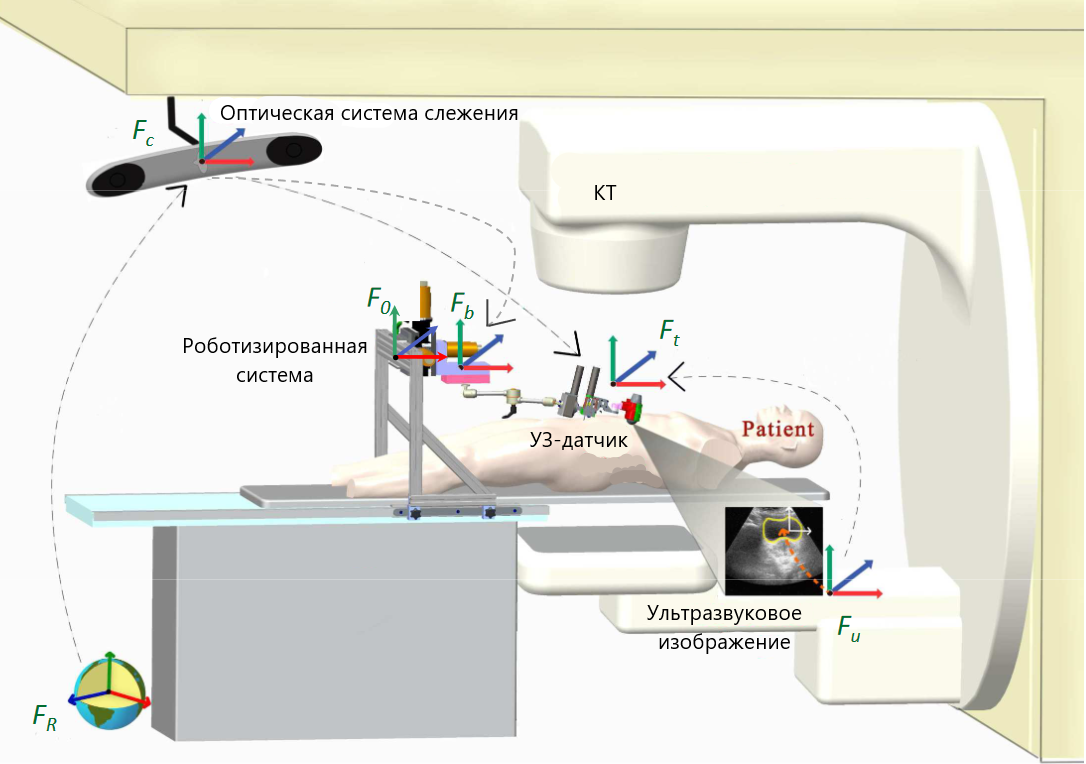
\includegraphics[width=0.7\textwidth]{Рисунки/система слежения.png}
\caption{\centering \onehalfspacing {Комплекс с роботизированной системой для проведения лучевой терапии \cite{litlink8}}}
\label{част}
\end{center}
\end{figure}

\section{Описание модели биологического объекта}

Чаще всего, доступ хирургического инструмента к сосуду осуществляется через бедренную артерию в верхней части бедра, реже — через плечевую, лучевую, подколенную и другие артерии. Поэтому объектом исследования является бедренная артерия, которая состоит из трех слоев: наружного, гладкомышечного слоя и эндотелия. На рисунке 1.4 изображены система артерий нижних конечностей и расположение бедренной артерии в ней.

\begin{figure}[!h]
\begin{center}
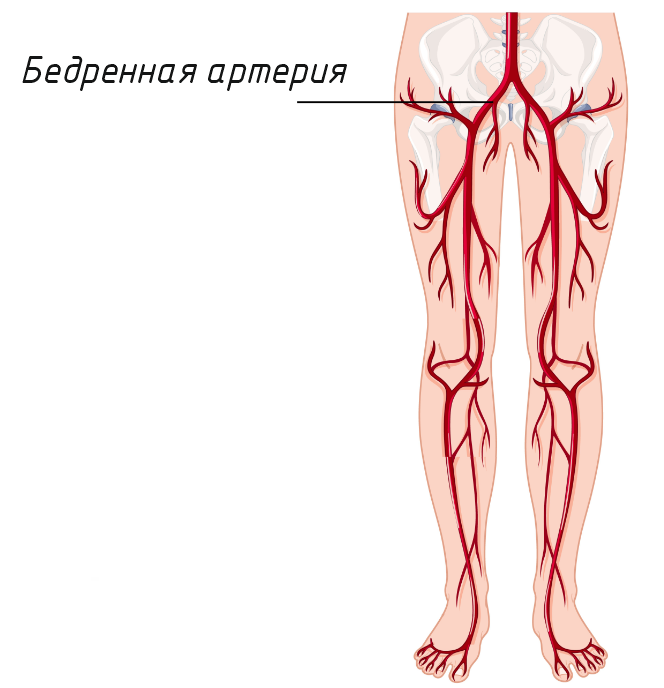
\includegraphics[width=0.4\textwidth]{Рисунки/бедренная артерия.png}
\caption{\centering \onehalfspacing {Локализация бедренной артерии в нижних конечностях}}
\label{част}
\end{center}
\end{figure}

Образование тромбов, сгустков крови в кровеносном сосуде, является самой распространенной проблемой, связанной с артериальными сосудами. Острый артериальный тромбоз является непосредственной причиной большинства случаев инфаркта миокарда (сердечного приступа) и примерно 80\% инсультов, что в совокупности является наиболее распространенной причиной смерти. На рисунке показана схема образования тромбоза в сосудистом русле \cite{litlink9}.

Первичным триггером артериального тромбоза является разрыв атеросклеротической бляшки, которая развивается за счет накопления липидных отложений и липид-нагруженных макрофагов (пенистых клеток) в стенке артерии \cite{litlink9}. Тромбы, которые образуются при разрыве бляшки, богаты тромбоцитами, которые представляют собой маленькие (около 1 мкм в диаметре) безъядерные клетки. Эти дискообразные клетки циркулируют в крови и образуют первичную гемостатическую пробку в местах повреждения сосудов. Если тромб оторвался от стенки сосуда его называют эмболой. На рисунке 1.5 схематично показано сосудистое русло артерии при нормальном кровотоке и при артериальном тромбозе.

\begin{figure}[!h]
\begin{center}
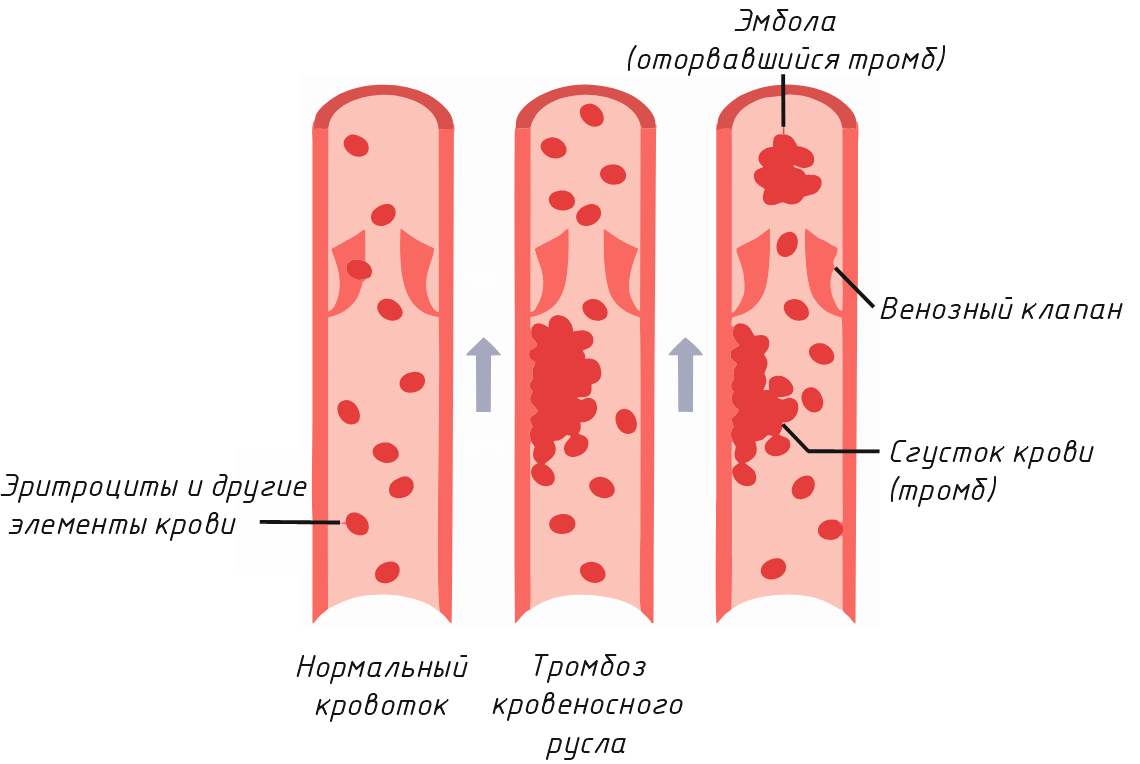
\includegraphics[width=0.8\textwidth]{Рисунки/тромбоз.png}
\caption{\centering \onehalfspacing {Сосудистое русло артерии при нормальном кровотоке и при артериальном тромбозе}}
\label{част}
\end{center}
\end{figure}

Отрыв тромбов может приводить к полной закупорке (тромбоэмболии) более мелких кровеносных сосудов. Процедуру хирургического удаления тромбов (тромбоэмболов) называют тромбоэктомией \cite{litlink10}. Оперативное вмешательство при эмболиях заключается в удалении эмбола катетером, сосудистыми кольцами, вакуум-отсосом или с помощью ретроградного промывания артерий. Наибольшую популярность среди них в последнее время получил метод эмболэктомии специальным баллонным катетером Фогарти. Его применение сделало операцию малотравматичной, простой и значительно повысило ее эффективность. Оперативные вмешательства при острых тромбозах принципиально отличаются от операций при эмболиях, они заключаются в том, что одновременно с тромбэктомией необходимо ликвидировать также причину заболевания, то есть выполнить ту или иную реконструкцию артерий \cite{litlink10}.

\section{Методы определения положения внутрисосудистых инструментов}

Диагностические и терапевтические процедуры под визуальным контролем стали обычной практикой для малоинвазивных вмешательств. Ультразвук, рентгеноскопия, магнитно-резонансная томография (МРТ) и компьютерная томография (КТ) используются для управления хирургическим инструментом во время вмешательства. Данные методы должны обеспечивать высокую точность, минимальную дозу ионизирующего облучения и доступность для использования в операционных.

\subsection{Рентгеновская визуализация}

Рентгеновская визуализация подразделяется на 4 вида: рентгенография, флюороскопия, ангиография и мультидетекторная КТ \cite{litlink11}. Все они имеют источник, детектор рентгеновского излучения и соответствующие системы управления. Каждый из этих методов, основанных на рентгеновских лучах, использует разные подвижные, как правило кольцевые, части томографического аппарата и детекторы \cite{litlink11}.

Рентгенография — исследование внутренней структуры организма, изображение которой создается при помощи рентгеновских лучей и проецируется на рентгеновскую пленку. Рентгенография позволяет рентгенологу не находиться в одной комнате с исследуемым во время включения рентгеновского аппарата и не подвергаться самому дополнительному облучению. Однако основным недостатком этого метода является невозможность оценить состояние организма при его функционировании. Рентгенограмма позволяет увидеть только функционирование в один момент времени.

Флюороскопия - это метод рентгенологического исследования, при котором изображение объекта получают на светящемся (флюоресцентном) экране. Этот метод используется для непосредственного наблюдения в режиме реального времени \cite{litlink12}. Его главное ограничение - невозможность четко визуализировать твердые органы из-за низкого пространственного разрешения. 

Ангиография - контрастное рентгенологическое исследование кровеносных сосудов, при котором в просвет сосуда вводится специальный контрастный материал и производится регистрация сигнала от контраста внешним считывающим устройством. Принцип метода состоит в том, что контрастный препарат заполняет внутренний просвет сосуда и, при наличии нарушения его проходимости, позволяет выявить область или точное место поражения сосуда.

Мультидетекторная компьютерная томография (МДКТ) отличается высокой точностью и скоростью проведения. Особенностью этого метода является то, что специальный излучатель рентгеновских лучей в томографе непрерывно вращается. МДКТ преобразует обычные аксиальные (перпендикулярные к срединной линии тела) срезы в трехмерное изображение.

Обычно эндоваскулярные вмешательства выполняются под контролем флюороскопии и цифровой субтракционной ангиографии, в основе которой лежит принцип компьютерного вычитания (субтракции) двух снимков до и после введения контрастного вещества в сосуд, чтобы визуализировать в реальном времени текущее положение хирургических инструментов \cite{litlink13}. Цифровая субтракционная ангиография используется для обеспечения правильного развертывания и положения стент-графта \cite{litlink11}.

Флюороскопия по-прежнему применяется при визуализации иглы во время биопсии легких, хотя во многих учреждениях ее использование почти полностью заменено КТ из-за ее более высокого разрешения. Она предпочтительнее, если пациент страдает ожирением \cite{litlink13}.

Благодаря быстрому получению данных, высокому разрешению, хорошей доступности и низкой стоимости, КТ является одним из лучших методов для процедур с визуальным контролем \cite{litlink14}. Из методов, основанных на рентгеновских лучах, КТ является самой востребованной из всех интервенционных процедур, требующих получения изображения поперечного сечения исследуемого объекта и широко используется для визуального контроля. Она предпочтительнее флюороскопии, МРТ и ультразвука из-за доступности, отсутствия серьезных противопоказаний, простоты использования и визуализации с высоким пространственным разрешением \cite{litlink11}.

Для повышения точности и уменьшения рентгеновского облучения при вмешательствах под контролем КТ был разработан ряд навигационных систем \cite{litlink15}. Некоторые системы были клинически протестированы в ходе сравнительных \cite{litlink16, litlink17} и рандомизированных исследований \cite{litlink18}. Эти навигационные системы включают локатор (оптический или электромагнитный), который отслеживает в реальном времени положение иглы. В статье \cite{litlink14} описаны результаты рандомизированного клинического исследования по оценке прототипа электромагнитной навигационной системы IMACTIS CT (Imactis SAS, Ла Тронш, Франция). Эта система позволяет интервенционному радиологу визуализировать запланированную траекторию движения иглы до ее введения в реальном времени (рисунок 1.6).

\begin{figure}[!h]
\begin{center}
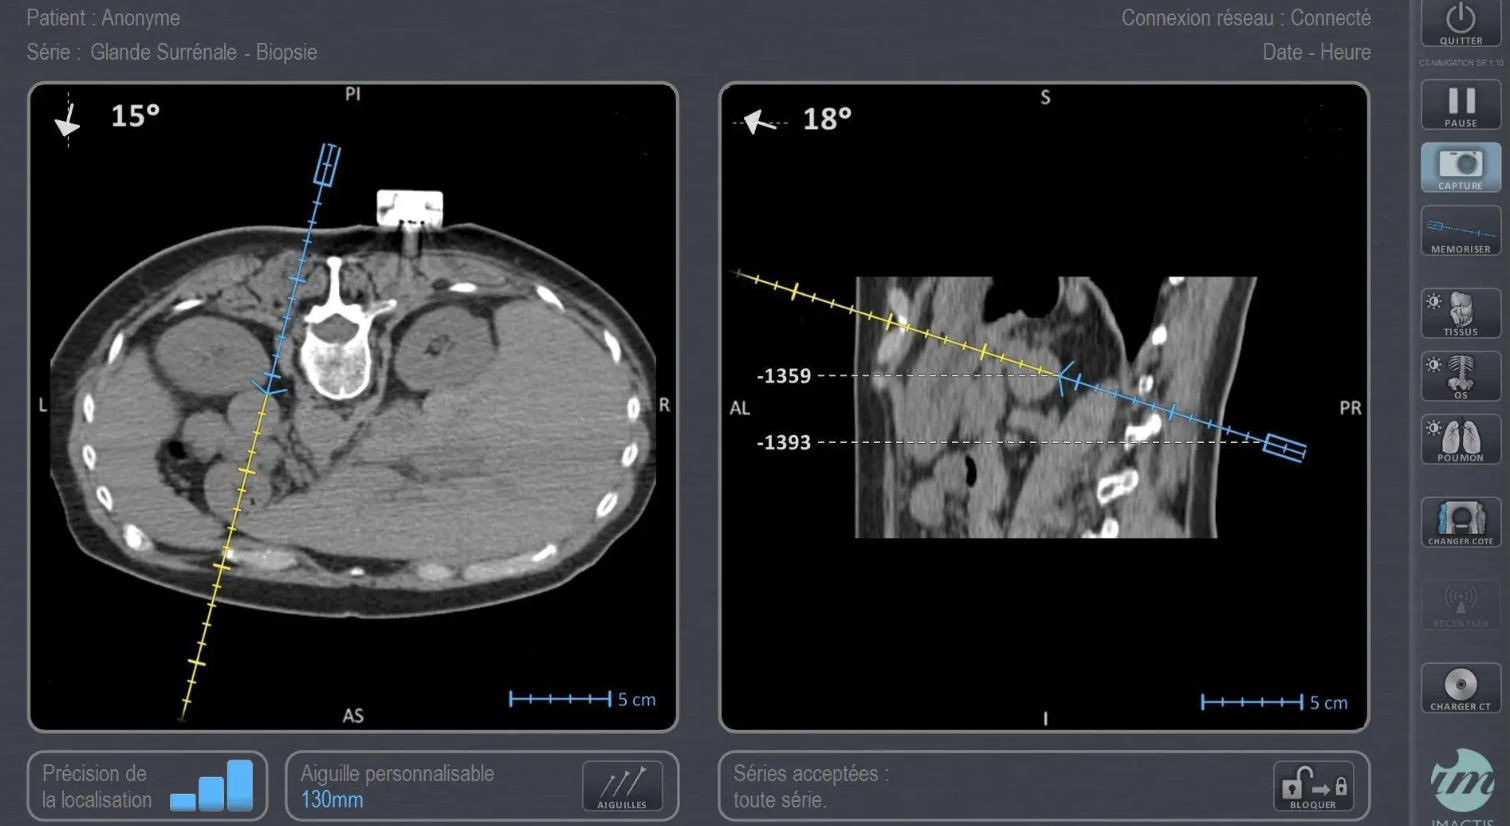
\includegraphics[width=0.8\textwidth]{Рисунки/КТ.png}
\caption{\centering \onehalfspacing {Изображение с навигационной системы IMACTIS
CT-NAVIGATION \cite{litlink14}}}
\label{част}
\end{center}
\end{figure}

Результаты исследования систем показали, что с помощью данной навигационной системы можно достичь выигрыша во времени и точности (до 4,1 мм) по сравнению со стандартным вмешательством под контролем КТ (точность до 8,9 мм).

В последнее время при хирургических вмешательствах с помощью КТ используется преимущественно настольная КТ. Томография с использованием С-образной дуги (С-дуга), которая включает в себя как источник рентгеновского излучения, так и детекторы, вращающей вокруг пациента и создающей
трехмерный набор изображений, подобных КТ (рисунок 1.7) \cite{litlink19,litlink20}.

\begin{figure}[!h]
\begin{center}
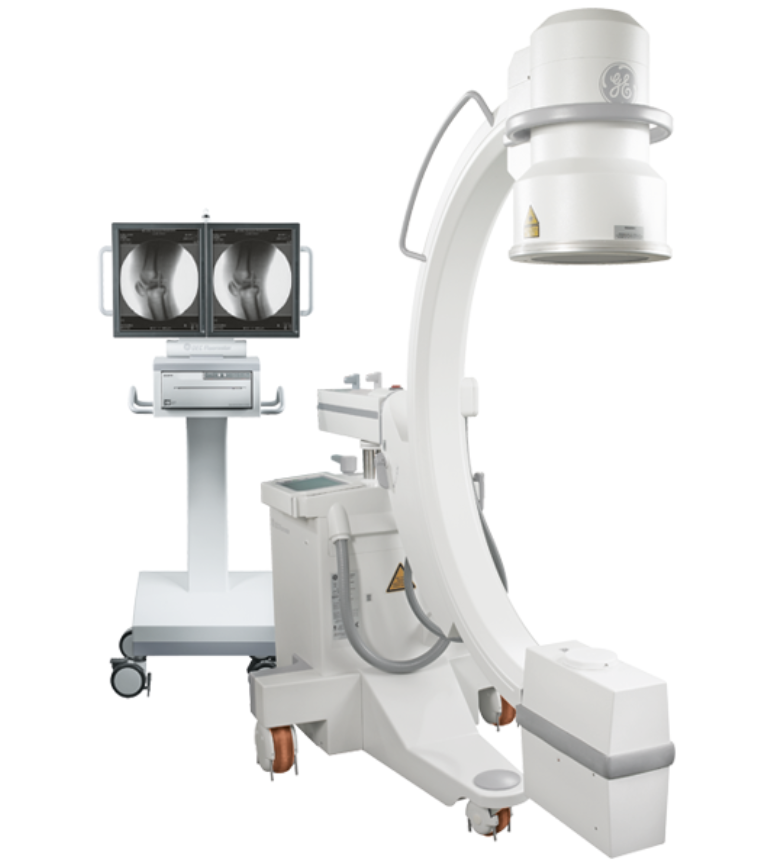
\includegraphics[width=0.5\textwidth]{Рисунки/КТ2.png}
\caption{\centering \onehalfspacing {Аппарат OEC Fluorostar Compact}}
\label{част}
\end{center}
\end{figure}

При сосудистых вмешательствах С-дуга используется для оценки относительного положения инструментов по сравнению с рассматриваемой анатомией \cite{litlink11}. Данный метод позволяет получать изображения в реальном времени с частотой кадров 25–30 кадров/с. КТ с C-дугой имеет лучшую визуализацию металлических артефактов по сравнению с традиционной КТ. Это может быть преимуществом при использовании данного метода визуализации при внутрисосудистом развертывании стента. Однако динамический диапазон получаемого изображения ограничивается 8–10 битами на пиксель (при традиционном КТ 14-16 бит на пиксель) \cite{litlink19}. Следовательно, могут быть визуализированы только высококонтрастные структуры, такие как сосуды и кости.

К недостаткам КТ относится введение йодсодержащего контрастного вещества, которое может вызвать аллергические реакции или почечную недостаточность. Кроме того, стоимость и наличие ионизирующего излучения ограничивают ее использование для длительного наблюдения. Также отсутствие контроля в реальном времени во время продвижения инструмента является серьезным недостатком. Чтобы его исключить, используются другие системы, такие как КТ-рентгеноскопия, конусно-лучевая компьютерная томография. Хотя они обеспечивают режим контроля в реальном времени, доза облучения при этом увеличивается \cite{litlink15}.

\subsection{Магнитно-резонансная томография}

Во многих медицинских центрах по всему миру проводятся эндоваскулярные процедуры под контролем МРТ. Высокий потенциал эндоваскулярной интервенционной МРТ объясняется тем, что она сочетает в себе трехмерную анатомическую визуализацию и определение локализации хирургического инструмента. Однако недостатками являются высокая стоимость томографа и акустический шум во время визуализации \cite{litlink21}. 

МРТ предоставляет анатомическую информацию о ткани-мишени с меньшим пространственным и временным разрешением по сравнению с рентгенографией. Интраоперационная МРТ дает возможность коррекции навигационных данных по ходу операции и повышает качество хирургического вмешательства, однако требует специального оборудования операционной, немагнитных аппаратов и инструментов. Низкопольные портативные МР-томографы требуют большего времени сканирования из-за низкой разрешающей способности, что увеличивает время операции и не позволяет проводить дополнительные исследования кровотока по ходу операции \cite{litlink22}.

Диагностические МРТ-сканеры высокого поля (от 1,0 до 1,5 Тл) не предназначены для интервенционного использования \cite{litlink23}. Было разработано несколько открытых интервенционных МРТ-сканеров с низким полем (от 0,064 до 0,5 Тл), но временное и пространственное разрешение, достигаемое с помощью таких сканеров, недостаточно для проведения эндоваскулярных процедур или получения точной функциональной информации.

Для отслеживания эндоваскулярных устройств было предложено несколько методов (рисунок 1.8).

\begin{figure}[!h]
\begin{center}
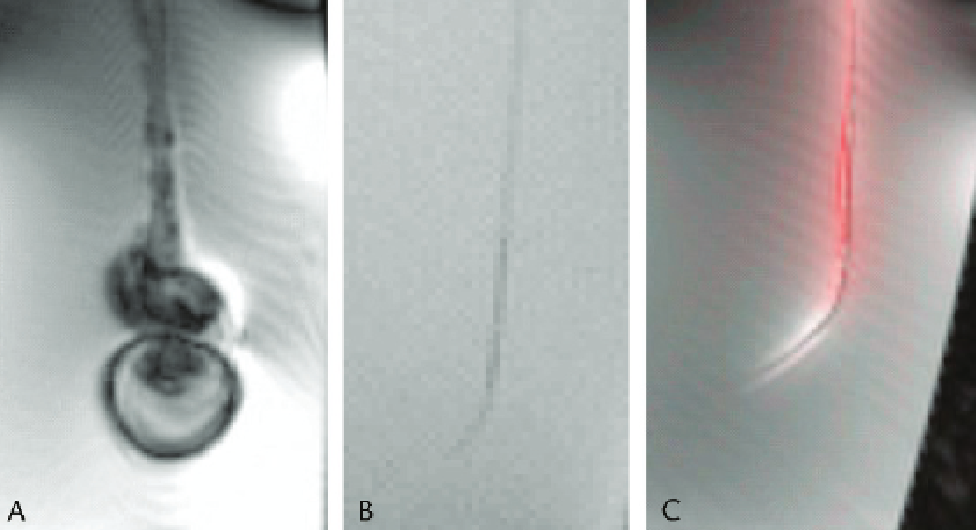
\includegraphics[width=0.8\textwidth]{Рисунки/МРТ.png}
\caption{\centering \onehalfspacing {Изображения катетеров различных конструкций для эндоваскулярных вмешательств под МРТ. A - пассивный рентгеновский
катетер с оплеткой из нержавеющей стали, вызывающий значительные
артефакты изображения. B - тот же катетер без стальной оплетки, что
делает его почти незаметным на изображении. C - активный катетер c
приемной катушкой \cite{litlink21}}}
\label{част}
\end{center}
\end{figure}

В так называемом «пассивном подходе» катетеры изготавливают из ферромагнитных материалов, чтобы увеличить их контраст на изображении \cite{litlink24}. Такие методы визуализации применяются при биопсии, а также подходят для вмешательств с использованием катетера. В отличие от жестких прямых биопсийных игл, которые можно полностью визуализировать на одном изображении, полученном вдоль стержня иглы, ангиографические катетеры гораздо более гибкие, что позволяет им повторять форму сосудов внутри человеческого тела. Следовательно, невозможно визуализировать весь ангиографический катетер с помощью метода визуализации, основанного на одном срезе. Хотя кончик катетера является основной целью для отслеживания, весь катетер должен постоянно визуализироваться во время вмешательства.

Другой подход к визуализации инструмента заключается в использовании проволоки в качестве приемной катушки. В «активном подходе» радиочастотные сигналы принимаются одной или несколькими микрокатушками \cite{litlink24}, встроенными в интервенционное устройство. Схема настроена на частоту МРТ-сканера. Эти сигналы отправляются в один из каналов приемника системы МРТ, где они оцифровываются и затем используются для определения положения катушки приемника в магните. Положение катушки может отображаться у оператора в виде курсора, наложенного на предварительно полученное статическое изображение.

В рамках исследования \cite{litlink25} была разработана и изготовлена двухэлементная катетерная фазированная (с электронным сканированием) матрица для активного отслеживания и визуализации стенок сосудов с высоким разрешением. Продвижение и втягивание катетера было успешно отслежено как в экспериментах с фантомом сосудов, так и в экспериментах по визуализации на свиньях. Отслеживание инструмента (местоположение и ориентация) были признаны работающими очень надежно и точно в более чем 1000 кадрах отслеживания/визуализации. Успешная локализация определялась, когда центр среза был размещен в пределах 2 мм от катушек слежения, а ориентация среза содержала в себе обе соленоидные катушки. Измеренная частота успеха составила 100\% для неподвижного катетера и > 97\% для движущегося катетера со скоростью до 3 см/с в аорте. В экспериментах с фантомом in vivo точность смещения оказалась больше, чем 2 мм, а точность ориентации среза больше, чем 2°. На изображениях стенки сосуда разрешение 240 мкм было достигнуто при времени экспозиции 15 с/срез. Артефактов, ухудшающих внешний вид стенки сосуда, не наблюдалось. По сравнению с рентгеновской визуализацией, которая обычно использует изображения с разрешением 1024x1024 пикселя при 15 кадрах в секунду, типичное интервенционное МР-изображение будет составлять 192x128 пикселей при 8 кадрах в секунду \cite{litlink21}.

\subsection{Электромагнитная навигация}

С-дуги обеспечивают только 2D-проекцию, и, как следствие, отсутствие
восприятия глубины затрудняет визуальную оценку положения и ориентации
катетеров внутри сосудистой сети пациента \cite{litlink26}. Кроме того, во время процедуры врач должен выполнить несколько измерений и корректировок положения и ориентации С-образной дуги: плохие углы проецирования могут вызвать такие проблемы, как ложное сужение сосудов и обскурация (затемнение) сосудов из-за перекрывающих сосудов или костей. Кроме того, традиционными катетерами трудно управлять и контролировать, и, следовательно, существует риск таких осложнений, как расслоение или перфорация сосудов \cite{litlink26}.

Принцип действия систем электромагнитной навигации основан на том,
что специальный генератор (работающий на постоянном или переменном токе) создает вокруг пациента электромагнитное поле, являющееся системой координат, в котором находится хирургический инструмент, оснащенный встроенным электромагнитным сенсором, либо на котором зафиксирован специальный адаптер. Перемещение сенсора в пространстве изменяет характеристики поля в этой точке, что позволяет навигационной системе определять координаты инструмента. В исследовании \cite{litlink26} безрамной электромагнитной навигации была описана система, которая позволила отслеживать угол наклона и ориентацию в пространстве хирургического инструмента с установленным на нем электромагнитным сенсором с погрешностью в пределах 4 мм.

Была предложена компьютерная хирургическая навигационная система, способная объединить объемную информацию, извлеченную из данных 3D-ангиографии, с электромагнитным отслеживанием в реальном времени эндоваскулярных инструментов: таким образом, хирург может следить за движением катетеров внутри трехмерной модели сосудистой сети пациента, не требуя получения флюороскопических изображений в реальном времени.

Максимальная такой визуализирующей системы составила 1,7 мм за серию из 70 измерений и средняя погрешность 1, 2 ± 0, 3 мм. Эти ошибки связаны с точностью калибровки проводника, точностью процедуры калибровки С-образной дуги и точностью локализации электромагнитной системы внутри операционной. Точность электромагнитных датчиков с пятью степенями свободы составляет 0,9 мм. Полученную точность можно считать достаточной для канюлирования большей части висцеральных ветвей брюшной аорты, которые у взрослых имеют средний диаметр в два раза больше, чем максимальная ошибка (т.е. чревная артерия 6, 4 ± 1, 1 мм, верхняя брыжеечная артерия 7, 3 ± 1, 4 мм, правая почечная артерия 5, 2 ± 1, 3 мм, левая почечная артерия 5, 1 ± 1, 0 мм).

На рынке представлена еще одна система электромагнитного трекинга Aurora (рисунок 1.9), создающая электромагнитное поле, в котором отслеживаются электромагнитные микродатчики. Она обеспечивает беспрепятственный трекинг датчиков, которые могут быть встроены в жесткие и гибкие медицинские инструменты, такие как ультразвуковые датчики, эндоскопы, катетеры \cite{litlink27}.

\begin{figure}[!h]
\begin{center}
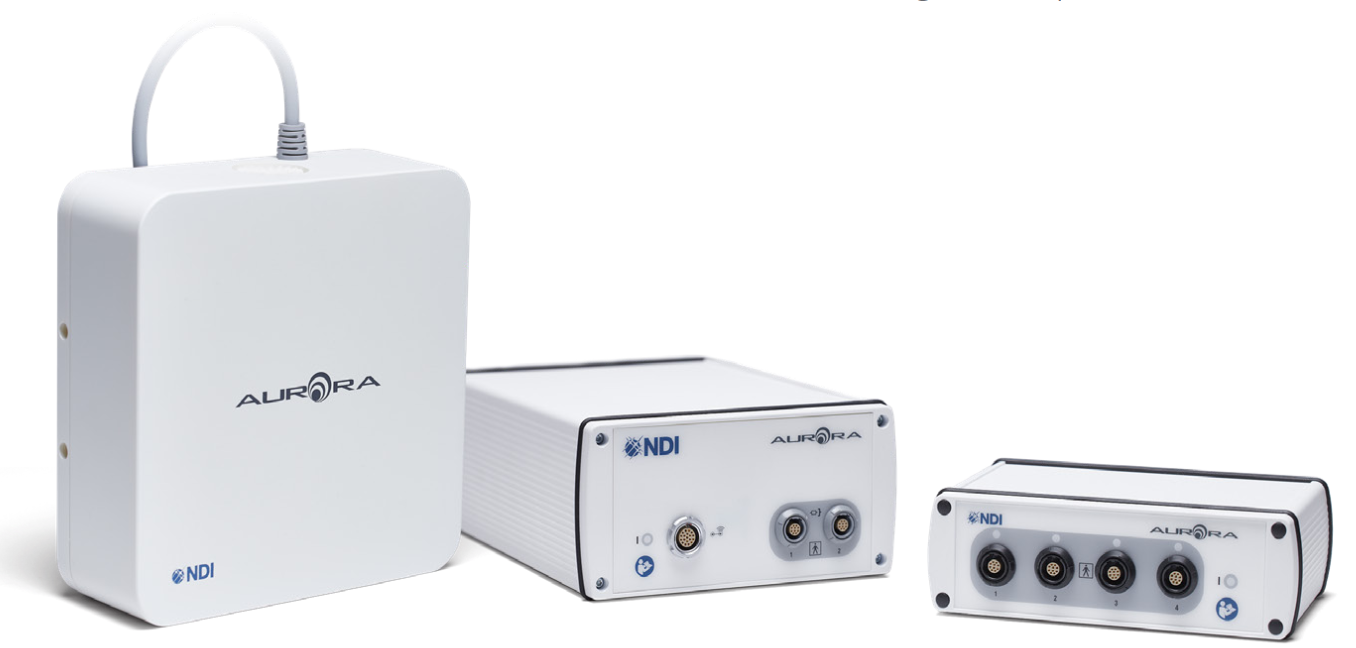
\includegraphics[width=0.8\textwidth]{Рисунки/Аврора.png}
\caption{\centering \onehalfspacing {Электромагнитная система трекинга Aurora \cite{litlink27}}}
\label{част}
\end{center}
\end{figure}

Непрерывное электромагнитное отслеживание инструментов может свести к минимуму потребность в интраоперационной рентгеноскопии, что может повысить безопасность и эффективность операции.

\subsection{Ультразвуковое исследование (УЗИ)}

Ультразвук распространенный метод трекинга инструмента при минимально инвазивных вмешательствах благодаря своей портативности и безопасности \cite{litlink28}. Основным его преимуществом перед другими передовыми методами визуализации (МРТ, компьютерная томографическая ангиография) является мобильность и работа в режиме реального времени \cite{litlink29}. Учитывая большее поле зрения, обеспечиваемое трехмерной визуализацией в реальном времени по сравнению с традиционной двумерной визуализацией, могут быть возможны более сложные процедуры под ультразвуковым контролем \cite{litlink30}. Особый интерес представляют процедуры, при которых хирургические инструменты и тканевые структуры визуализируются одновременно для достижения точных манипуляций.

Для медицинской диагностики УЗИ визуализация имеет хорошее разрешение для мягких тканей, портативность и применимость в широком диапазоне клинических условий с минимальными затратами. С помощью современных систем УЗИ возможно одновременно визуализировать жесткий наконечник инструмента (например, биопсийная игла), который направлен к удаленной цели, и саму цель \cite{litlink31}. Они включают в себя интегрирование 2D-УЗИ изображений в 3D-операционную систему с дополненной реальностью \cite{litlink32}, добавление устройства магнитного слежения к двумерному ультразвуковому датчику для предоставления дополнительных навигационных сигналов \cite{litlink33}, использование роботизированной руки для компьютерного позиционирования
биопсийной иглы под контролем УЗИ \cite{litlink34}. УЗИ предпочтительнее использовать из-за высокой частоты кадров и отсутствия излучения.

\section{Методы трекинга внутрисосудистых инструментов на изображениях с ультразвуковых визуализационных систем}

Оптическое отслеживание обеспечивает высокую точность, но требует
наличия прямой видимости между оптическими датчиками и камерой отслеживания. В результате все отслеживание положения инструмента должно выполняться снаружи. В этом случае ошибки отслеживания ориентации инструмента приводят к неверному определению положения наконечника инструмента \cite{litlink30}.

Известно, что сложные хирургические задачи с использованием двух инструментов, невозможные с 2D-контролем УЗИ, могут быть выполнены с помощью 3D УЗИ-визуализации в реальном времени с результатами, сопоставимыми с результатами, полученными с помощью оптических изображений. Для получения ультразвуковых изображений выбранной области интереса датчик необходимо расположить перпендикулярно поверхности \cite{litlink35}. 

Точка введения инструмента и траектория рассчитываются с учетом того, что ультразвуковой датчик расположен перпендикулярно поверхности пациента, а инструмент и цель находятся в одной плоскости. Из соображений безопасности инструмент может проходить только через ткань, которая уже была визуализирована.

Планирование траектории осуществляется путем проецирования области интереса на поверхность пациента. Перед получением УЗ-изображения оператор наносит достаточное количество ультразвукового геля для достижения акустической связи. Затем двумерные ультразвуковые изображения записываются одновременно с данными механического отслеживания, предоставляемыми роботизированной системой. После того, как данные записаны, изображения обрабатывают с помощью четырехсторонней интерполяции, добиваясь компромисса между вычислительной производительностью и качеством изображения.

Проблемой ультразвуковой визуализации является плохая видимость инструмента вследствие существенной разницы как в импедансе и абсорбции между биологическими тканями и инструментами, что приводит к разнообразным артефактам изображения \cite{litlink36}. С точки зрения их влияния на изображение, артефакты можно сгруппировать в три типа: артефакты сглаживания формы, в которых не видны детали формы инструмента, артефакты выпадения, в которых части инструмента появляются и исчезают при его перемещении, и топологические артефакты, изменяющие форму инструмента. Эти три типа артефактов в совокупности скрывают как геометрические детали инструмента, так и его относительное расположение относительно ткани.

В так называемом активном отслеживании применяются датчики для
определения положения инструмента с использованием ультразвукового изображения \cite{litlink30}. Приемник ультразвука, который установлен на катетере для определения интенсивности и направления ультразвукового луча, показывает положение катетера на изображении \cite{litlink37}. С помощью этого метода достигнута допустимая точность в экспериментах in vitro с различными расстояниями между катетером и ультразвуковым преобразователем, однако для определения ориентации инструмента требуется несколько электромагнитных датчиков.

В работе \cite{litlink38} представлена методика, способная обнаруживать инструменты, используемые в минимально инвазивных процедурах, такие как эндоскопические захваты, катетеры, режущие устройства. Инструменты, используемые при минимально инвазивных процедурах, имеют цилиндрическую форму и обычно диаметром 3–10 мм. Первый шаг - определить ось инструмента, для используются преобразования Радона (рисунок 1.10) \cite{litlink38}. Математическая запись преобразования Радона показана в формуле 1.1.

\begin{figure}[!h]
\begin{center}
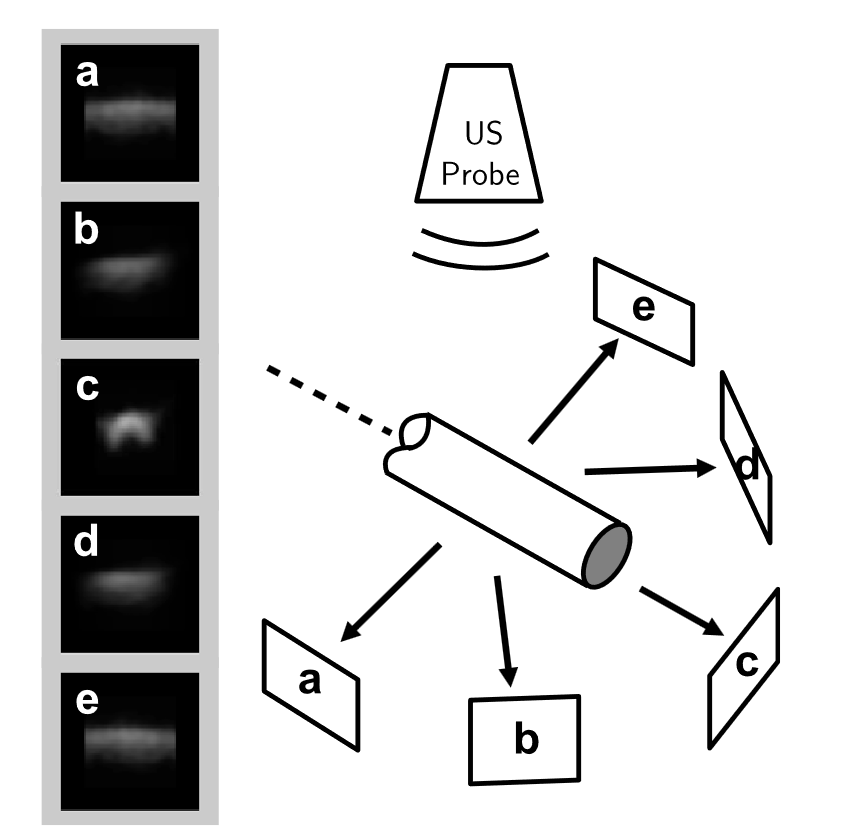
\includegraphics[width=0.5\textwidth]{Рисунки/трэкинг.png}
\caption{\centering \onehalfspacing {Обнаружение оси инструмента с помощью преобразования Радона. Каждое изображение (a – e) представляет собой проекцию
ультразвукового изображения в соответствующем направлении,
показанном на схеме. Проекция по оси инструмента (c) самая яркая}}
\label{част}
\end{center}
\end{figure}

\begin{equation}
\check{g}(\theta, \phi, u, v)=\int g(s \tau(\theta, \phi)+u \alpha(\theta, \phi)+v \beta(\theta, \phi)) d s
\end{equation}

где $\check{g}$ - модифицированное радоновое пространство ультразвукового объема g. Каждая точка в $\check{g}$ соответствует интегралу по трехмерной линии, определяемой четырьмя параметрами $\theta$, $\phi$, $v$ и $u$. Угловые параметры $\theta$ и $\phi$ (рисунок 1.11) \cite{litlink38} определяют ортонормированный базис, состоящий из $\alpha$, $\beta$ и $\tau$, который определяются как:

\begin{equation}
\tau=\left(\begin{array}{c}
\cos \theta \cos \phi \\
\sin \theta \cos \phi \\
\sin \phi
\end{array}\right), \alpha=\left(\begin{array}{c}
-\sin \theta \\
\cos \theta \\
0
\end{array}\right), \beta=\left(\begin{array}{c}
-\cos \theta \sin \phi \\
-\sin \theta \sin \phi \\
\cos \theta
\end{array}\right)
\end{equation}

\begin{figure}[!h]
\begin{center}
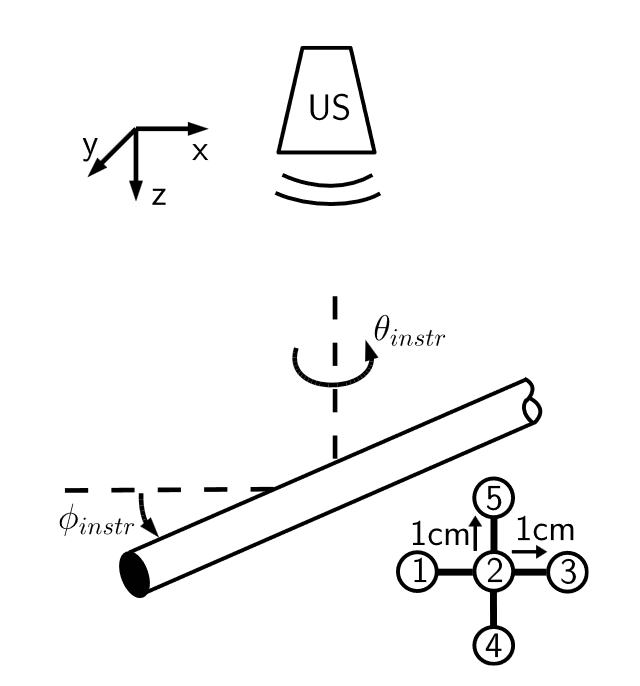
\includegraphics[width=0.5\textwidth]{Рисунки/угловые.png}
\caption{\centering \onehalfspacing {Параметры положения инструмента}}
\label{част}
\end{center}
\end{figure}

Два позиционных параметра $u$ и $v$ также используются для определения трехмерной линии. Идентификация линий в трехмерном объеме является проблемой поиска локальных максимумов $\check{g}$. При нахождении максимального значения $\check{g}$ ось инструмента в трехмерном пространстве неявно определяется параметрами ($\theta$, $\phi$, $v$ и $u$). Этот алгоритм особенно хорошо подходит для реализации в параллельных архитектурах, таких как современные графические процессоры. В первоначальной реализации он обнаруживал инструменты на ультразвуковых изображениях за 0,6 с. Чтобы улучшить эту реализацию, был усовершенствован алгоритм поиска, который определяет максимумы уравнения 1.1.

Пространство $g$ дискретизируется с шагом 5 вокселей по x, y и z. Для углов $\theta$ и $\phi$ оно дискретизируется с шагом 10 градусов. Из-за симметрии углы выбираются только от 0 до 180 градусов. Эта процедура представляет собой инициализацию отслеживания инструмента, так как поиск инструмента выполняется по всему объему. Для объемов вокселей 148x48x208 это приводит к 408 000 итерациям уравнения 1.1. Для последующих кадров алгоритм отслеживания ограничивает пространство поиска областью с центром в местоположении, найденном в предыдущем кадре. Поскольку ультразвуковые изображения обновляются с частотой 25–28 Гц, это пространство поиска может быть довольно небольшим.

В экспериментах обнаружено, что ограничение пространства поиска до ±5 вокселей в направлениях x, y и z и ± 10 градусов вокруг углов $\theta$ и $\phi$ (рисунок 1.11), найденных в предыдущем кадре, достаточно для захвата типичных хирургических движений. После того, как $\check{g}$ будет отобран в достаточной степени, максимум определяет положение оси инструмента.

\section{Сравнительный анализ существующих роботизированных систем c хирургическим и визуализирующим манипуляторами}

При проектировании роботизированной конструкции для ультразвуковой визуализации необходимо учитывать несколько параметров: минимальное рабочее пространство, точность перемещения датчика, легкая конструкция (менее 3 кг, которую может выдержать пациент), компактность робота для облегчения обследования и транспортировки \cite{litlink39}. Системы с двумя роботами-манипуляторами обеспечивают лучшую гибкость, чем системы с одним роботом, но их настройка сложнее в реализации.

Ronna G4  — роботизированная нейронавигационная система на основе шарнирных роботов-манипуляторов, предназначенная для минимально инвазивных стереотаксических процедур, таких как биопсия, стереоэлектроэнцефалография, хирургия эпилепсии и резекция опухолей (рисунок 1.12) \cite{litlink40}. Ronna может быть сконфигурирована как система с одним манипулятором, так и с двумя: одноплечевая система предназначена для стереотаксической нейронавигации и служит помощником хирурга в навигации, а двухплечевая конфигурация выполняет автономные инвазивные операционные задачи, такие как сверление кости, введение зонда или иглы и т.д. 

\begin{figure}[!h]
\begin{center}
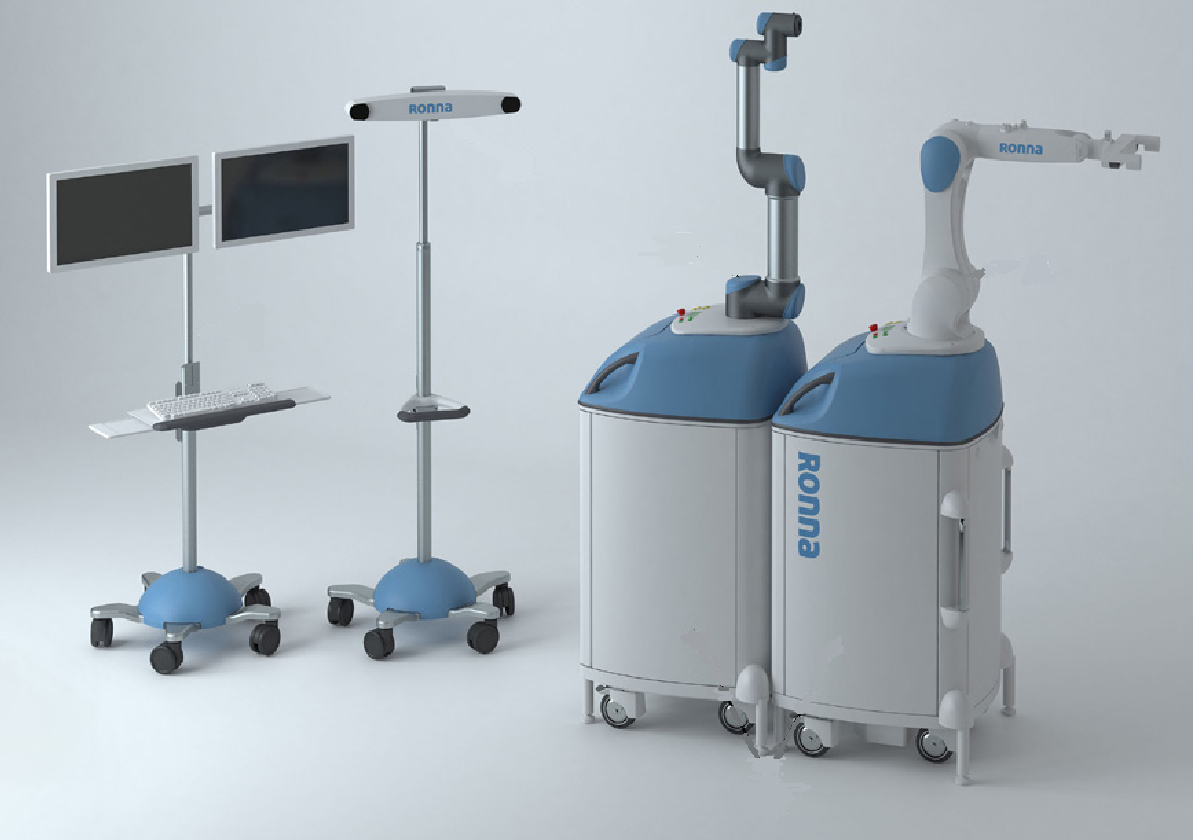
\includegraphics[width=0.7\textwidth]{Рисунки/RONNA G4.png}
\caption{\centering \onehalfspacing {Роботизированная нейронавигационная система Ronna G4 \cite{litlink40}}}
\label{част}
\end{center}
\end{figure}

Визуализирующий манипулятор управляет двумя инфракрасными камерами с макрообъективами, расположенными под углом 55° в одной плоскости. Хирургический манипулятор предназначен для автоматизированного роботизированного сверления костей и манипуляции хирургическими инструментами. Он устанавливает операционный инструмент в направляющую инструмента, указывая на рабочую точку.

Ronna обладает автоматизированным планированием положения робота и точным наведением инструмента. Система обеспечивает позиционирование хирургического инструмента во внутричерепном пространстве пациента. С 2016 года система проходит клинические испытания в университетской клинике Хорватии.

Для задач по введению иглы, таких как биопсия, предложена автоматизированная система с двумя роботами \cite{litlink35}. Система может выполнять как ультразвуковую визуализацию, так и хирургическое вмешательство. В ней используются два робота Kuka LBR iiwa, один из которых держит иглу, а другой — ультразвуковой датчик (рисунок 1.13). Визуализирующий робот позволяет контролировать силу прижатия датчика. Данные прединтервенционного планирования регистрируются в системе координат робота на этапе инициализации с использованием регистрации изображений. Врач выбирает область интереса на изображениях поверхности пациентов, полученных с помощью RGB-камер, установленных на роботах. Роботы перемещают ультразвуковой датчик и иглу в область интереса и начинают отслеживание цели на основе предварительно определенной цели, а также отслеживание иглы для введения иглы в соответствии с планом. Данная система была испытана на фантоме из желатина.

\begin{figure}[!h]
\begin{center}
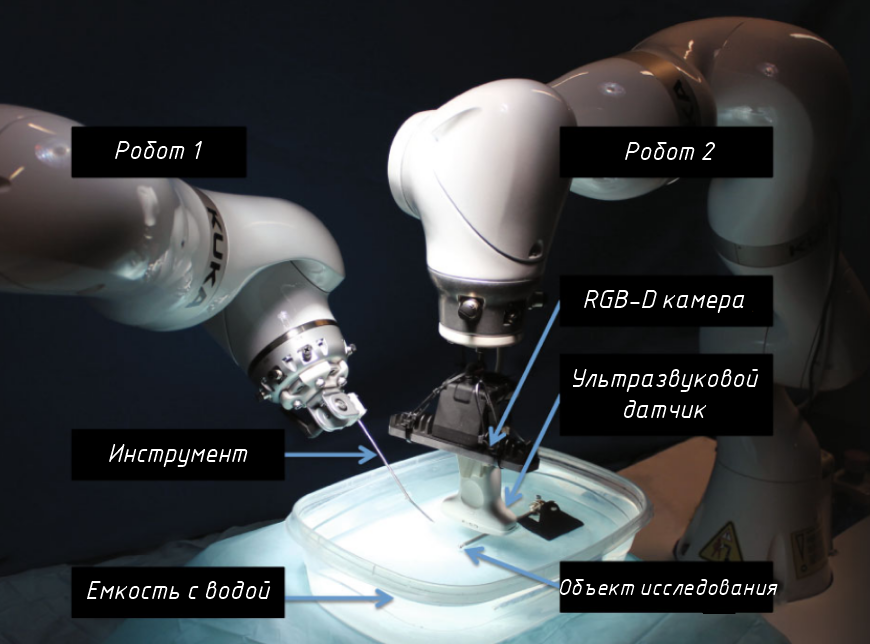
\includegraphics[width=0.7\textwidth]{Рисунки/аналог1.png}
\caption{\centering \onehalfspacing {Манипуляторы Kuka LBR iiwa, удерживающие инструмент и ультразвуковой датчик \cite{litlink41}}}
\label{част}
\end{center}
\end{figure}
\newpage

В исследовании \cite{litlink41} была разработана система для введения гибких игл под ультразвуковым контролем (рисунок 1.14). Основное преимущество данной системы заключается в том, что иглу можно точно направить к цели без необходимости выполнять многократные повторные введения, что сокращает продолжительность вмешательства. Для проведения экспериментов была использована гибкая игла со скошенным концом, прикрепленная к концевому эффектору робота Viper S650 с 6 степенями свободы (Adept Technology Inc., США). Иглу вводилась в самодельный желатиновый фантом, имитирующий мягкие ткани. Ультразвуковой контроль производится с помощью ультразвукового датчика 4DC7-3/40 3D (Ultrasonix Medical Corporation, Канада), который находится в неподвижном состоянии.   Обработка изображений выполняется на рабочей станции (Intel Core i7, NVIDIA Quadro K2000), которая получает данные от ультразвуковой системы SonixTouch и обеспечивает связь с роботом. В результате врачу отображаются два ортогональных среза, на которых выделено текущее положение иглы.

\begin{figure}[!h]
\begin{center}
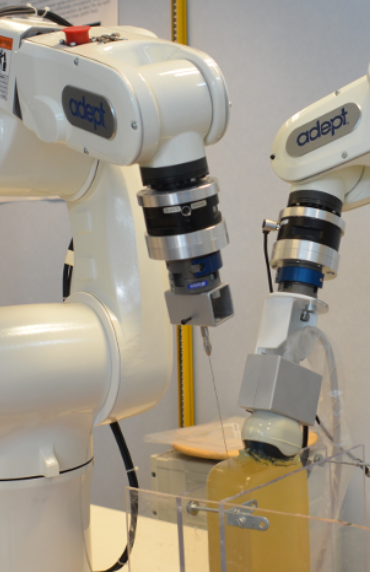
\includegraphics[width=0.4\textwidth]{Рисунки/аналог3.png}
\caption{\centering \onehalfspacing {Система из двух манипуляторов Viper S650 (Adept): хирургическим с гибкой иглой и визуализирующим с ультразвуковым датчиком}}
\label{част}
\end{center}
\end{figure}

В исследовании \cite{litlink42} создан прототип, состоящих из двух манипуляторов с шестью степенями свободы для проведения почечной пункции (рисунок 1.15). Один манипулятор выполняет ультразвуковое сканирование, другой - почечную пункцию. Оба робота-манипулятора имеют функцию позиционирования и функцию управления. Перед началом операции врач размещает два манипулятора у почки пациента и точки входа иглы. 

Сообщается, что испытания на животных подтверждают эффективность прототипа системы.
В будущем такая роботизированная система пункции может быть использована для клинических испытаний, что, как ожидается, позволит лучше контролировать смещение почек, вызванное дыханием в процессе пункции. Это повысит успешность пункционной хирургии и снизит частоту осложнений, поэтому система имеет хорошие перспективы для применения.

\begin{figure}[!h]
\begin{center}
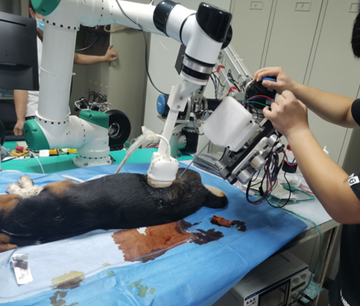
\includegraphics[width=0.6\textwidth]{Рисунки/аналог4.png}
\caption{\centering \onehalfspacing {Прототип роботизированной системы \cite{litlink42}}}
\label{част}
\end{center}
\end{figure}
\newpage

\section{Обзор существующих материалов для изготовления фантома мягких тканей}

Ультразвуковые фантомы - это неоднородные среды с определенными геометрическими и механическими характеристиками, которые используются для настройки ультразвукового оборудования. Основная часть фантома представляет собой однородное вещество с акустическими свойствами, соответствующими свойствам тканей человека с точки зрения скорости звука:

\begin{equation}
\boldsymbol{c}=\sqrt{\frac{{E}}{{\rho}}},
\end{equation}

где ${E}$ - модуль Юнга;

$\rho$ - плотность вещества.

А также затухания (дБ/см):

\begin{equation}
\boldsymbol{\alpha}=\frac{-ln (A_{d}/A_{0})}{d},
\end{equation}

где $A_{0}$ и $A_{d}$ - амплитуды звуковых колебаний до прохождения через вещество и после соответственно;

$d$ - толщина образца.

Коэффициент затухания, измеряемый в дБ/(см*МГц), рассчитывается по формуле:

\begin{equation}
\boldsymbol{\alpha_{k}}=\frac{\boldsymbol{\alpha}}{f},
\end{equation}

где f - частота ультразвукового импульса.

Последний можно модифицировать, варьируя концентрацию мельчайших включений с различными реологическими свойствами \cite{litlink43}.

В исследовании \cite{litlink44} рекомендуется использовать фантомы со скоростью звука 1540 м/с и с коэффициентом затухания 0,5-0,7 дБ/(см*МГц) для частотного диапазона от 2 до 15 МГц. 

Мягкие ткани состоят из мышц, сухожилий, связок, фасций, жира, фиброзной ткани, синовиальных оболочек, нервов и кровеносных сосудов. В таблице 1.1 указаны наиболее характерные акустические свойства мягких тканей организма.

\begin{table}[h]
\captionsetup[table]{singlelinecheck=false,justification=raggedleft}
\ttabbox
{\caption {\onehalfspacing Диапазон значений акустических свойств мягких биологических тканей}}
{\begin{tabular}{| >{\centering\arraybackslash}m{1.1in} | >{\centering\arraybackslash}m{1.1in} | >{\centering\arraybackslash}m{1.2in} | >{\centering\arraybackslash}m{1.2in}| >{\centering\arraybackslash}m{1.1in}|}
\hline 
Ткань & Плотность, кг/м^3 & Скорость звука в среде, м/с &  Коэффициент затухания, дБ/(см*МГц) & Модуль Юнга, кПа \\ 
\hline
Кожа & 1100 & 1631 & 0,22 & 100-100000 \\
\hline
Жировая ткань & 916 & 1435 & 0,975 & 18-24\\
\hline
Мышечная ткань & 1041 & 1595 & 1,47 & 6-7 \\
\hline
\end{tabular}}
\end{table}

Одна из проблем при моделировании механических свойств мягкой ткани - воспроизвести вязкоупругое поведение фантомов, наблюдаемое в биологических тканях. Большинство биологических тканей демонстрируют зависящее от времени поведение напряжения-деформации, которое характерно для вязкоупругих материалов. Однако для небольших деформаций поведение можно считать упругим, а для узких диапазонов деформации модуль Юнга можно считать постоянным \cite{litlink44}. 

Материалы, соответствующие вышеописанным акустическим и механическим свойствам, делятся на три группы: гидрогели, силиконы и полидиметилсилоксаны (ПДМС). Свойства гидрогелей наиболее схожи со свойствами мягких тканей, но они нестабильны  и требуют трудоемкого производства. Силиконы часто используются в изготовлении фантомов вместе со специальными добавками, чтобы приблизить их свойства к мягким тканям. ПДМС является хорошей добавкой, а также основным компонентом для изготовления фантомов кровеносных сосудов.

\subsection{Акустические и механические свойства гидрогелей}

Гели на водной основе (гидрогели) - ультразвуковые фантомы, наиболее хорошо имитирующие мягкую ткань \cite{litlink45}. Однако модуль Юнга этих гелей сильно увеличивается с течением времени из-за сильной деформации образца и находится в диапазоне 10–110 кПа, что не соответствует значениям модуля Юнга мягких тканей 3-6 кПа. 

Среди наиболее распространенных материалов, используемых для изготовления самодельных фантомов и относящихся к семейству гидрогелей, являются агароза, желатин, поливиниловый спирт (ПВС) и полиакриламид (ПААГ).

В исследовании \cite{litlink46} в фантомах на основе желатина в качестве акустического рассеивающего материала использовался графит с концентрациями 5\%, 8\%, 10\% и 12,4\%. При увеличении концентрации графита коэффициент затухания увеличивается с 0,36 до 0,9 дБ/(см*МГц), а при концентрации 8\% скорость звука максимальна и равна 1540 м/c.

В \cite{litlink45} в качестве материала для фантома предлагается гель-сополимер в масле. Сополимеры типа стирол-этилен/бутилен-стирол смешиваются в минеральном масле с акустическими рассеивателями и дают мягкую эластичную полупрозрачную среду. Модуль Юнга составляет 5,2 кПа, что соответствует мягкой ткани. Этот материал однородный, простой в производстве, нетоксичный и недорогой. Однако исследования по использованию этого материала продолжаются.  

Одним из наиболее распространенных в медицинской визуализации материалов, имитирующих ткань, является агар. Его преимуществом является почти линейная зависимость затухания от частоты ультразвука. \cite{litlink46}. Агар-фантомы могут храниться в дистиллированной воде в течение длительного времени (более 3 месяцев) без изменения их акустических характеристик. Механические свойства изменяются в пределах 1-2\% за счет потери воды. Компонентами агарозной смеси обычно являются агар, N-пропанол и деионизированная вода. 

Основным недостатком агара является то, что при обычном лабораторном использовании его срок жизни часто ограничивается менее, чем одним месяцем из-за микробной инвазии и дегидратации \cite{litlink47}.

В работе \cite{litlink48} были исследованы биомеханические свойства образцов на основе агара для диапазона концентраций от 1,7\% до 6,6\%, а также измерены акустические параметры, такие как скорость звука, коэффициент затухания и акустический импеданс с использованием импульсного сигнала на частоте 5 МГц. Акустический импеданс рассчитывается по формуле:

\begin{equation}
Z=\rho \mathbf{c},
\end{equation}

где $\rho$ - плотность вещества,

$c$ - скорость звука.

Наблюдаемые значения модуля Юнга составили от 50 кПа до 450 кПа, что соответствует диапазону модуля Юнга в мягких биологических тканях. Увеличение концентрации агара привело к увеличению модуля Юнга. Скорость звука находилась в диапазоне от 1540 до 1671 м/с, а коэффициент затухания практически не менялся при изменении концентрации и был равен 0,75 дБ/(см*МГц). 

Показано  \cite{litlink49}, что фантом на агаровой основе c добавлением глицерина поддерживает соответствующие значения акустических параметров в диапазоне частот 17–23 МГц, увеличение концентрации глицерина приводит к снижению модуля Юнга, однако глицерин вымывается из образца, что влияет на скорость звука, если его поместить в воду  \cite{litlink50}. 

По сравнению с силиконом и полидиметилсилоксаном (ПДМС), модель из агарозного геля (рисунок 1.16b) превосходит два других материала \cite{litlink51}, так как она больше соответствует реальному органу. Фантомы из силиконового эластомера (рисунок 1.16с) и ПДМС (рисунок 1.16d) показали сильное размытие изображения, на рисунке можно увидеть только белый контур фантома. Заменители тканей на основе агарозы имеют ограниченный размер (обычно 5 см в толщину), потому что они должны иметь высокое отношение поверхности к объему для правильного отвердения \cite{litlink52}.

Из \cite{litlink44} также можно сделать вывод, что на частотном диапазоне ультразвука от 2 до 15 МГц (при температуре от 10 до 30$^{\circ}$ С) скорость звука в агаре изменяется не более, чем на 1,3\%, а коэффициент затухания остается постоянным. 

\begin{figure}[H]
\begin{center}
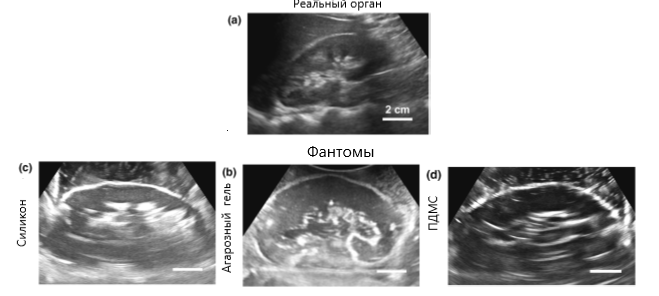
\includegraphics[width=0.9\textwidth]{Рисунки/УЗИ.png}
\caption{\centering Сравнение ультразвукового изображения фантомов из силикона, ПДМС и агарозного геля}.
\label{оболочка}
\end{center}
\end{figure}

В исследовании \cite{litlink53} используется другой тип гидрогелей - гелевый воск. Применяются две добавки к гелевому воску (углеводород с добавлением аполимера, модель FF1 003) - стеклянные сферы с номинальным диаметром от 0 до 63 мкм для увеличения акустического рассеяния и парафиновый воск для увеличения коэффициента затухания. Добавление парафина оказало сильное влияние на коэффициент затухания и слабое влияние на скорость звука и акустический импеданс. Коэффициент затухания быстро увеличивался с увеличением концентрации парафинового воска. Когда концентрация добавленного парафинового воска была увеличена до 8 \%, затухание увеличилось с 0,72 до 2,91 дБ/см на 3 МГц и на 10 МГц с 6,84 до 26,63 дБ/см. В том же диапазоне концентраций скорость звука существенно не изменилась. Скорость звука гелевого воска (1448,5 м/с) на 6,3 \% ниже, чем средняя скорость звука для мягких тканей (1540 м/с). Добавление стеклянных сфер для обеспечения обратного акустического рассеяния оказало заметное влияние на внешний вид ультразвука и не оказало существенного влияния на скорость звука и акустическое затухание.

Еще одним типом гидрогелей, используемых для изготовления фантома является ПВС. Фантомы на основе ПВС имеют низкую стоимость, неограниченный срок службы при хранении в воде, высокую структурную жесткость и требуют меньше ингредиентов по сравнению с более распространенными тканевыми заменителями на основе агарозы с добавками \cite{litlink54}. Однако довольно трудоемкая процедура подготовки этого материала является главным недостатком.

\subsection{ПДМС}

Фантомы ПДМС могут быть полезны для хирургического обучения, для моделирования таких процедур, как биопсия и введение иглы. Также ПДМС используется для имитации сосудов \cite{litlink54}. Но скорость звука и, следовательно, акустический импеданс ПДМС меньше по сравнению с тканью сосуда человека, что приводит к нехарактерным акустическим отражениям на стенке фантомного сосуда. Механические свойства ПДМС можно изменять, варьируя соотношение эластомера и отвердителя (например, изменив соотношение с 1:10 до 1: 5, скорость звука увеличится с 1076,5 до до 1119,5 м/с, а затухание снизится с 21,30 до 14,86 дБ/см на частоте 5 МГц) \cite{litlink55} или отверждая при различных температурах. 

\subsection{Силиконы}

Несмотря на распространенность агарозного геля, преимущественными материалами для фантома являются силиконовые материалы из-за их высокой прочности и простоты изготовления. Ниже будут рассмотрены свойства силиконов RTV615, Dragon Skin, Ecoflex 0010 и Ecoflex 0030. Эти силиконы обладают необходимыми механическими свойствами (способность сохранять свою форму, устойчивость к деградации), большим запасом прочности и уже испытывались в изготовлении фантомов.

Во всех силиконовых фантомах скорость звука составляет примерно 1000 м/с, и они имеют высокое затухание (обычно > 2 дБ/см). 

Фантомы из силиконов, в отличие от агара, стабильны в течение месяцев и даже лет и, в отличие от агара, нечувствительны к грубому обращению \cite{litlink56}. Как и агар, силикон не токсичен при приготовлении и применении. Время отверждения зависит марки силикона и от температуры, чем выше температура, тем меньше время отверждения. 

Из группы эластомеров, проанализированных в литературе, силиконовый каучук RTV615 является материалом с самым низким коэффициентом затухания (1,2-1,55 дБ/см*МГц), но его скорость звука равна 1080 м/с, что составляет 74\% от скорости звука в жировой ткани \cite{litlink46}. 

Dragon Skin –платиновый силикон с большой прочностью на разрыв, выдерживающий деформацию до 1000\%. \cite{litlink57}. Его главным преимуществом является то, что он имеет ту же скорость звука, что и мягкие ткани. Однако коэффициент затухания этого силикона немного выше по сравнению с тканями человека, что ограничивает глубину обзора при ультразвуковой визуализации.

В данный момент cиликоны Ecoflex представлены в четырех вариантах, различающихся степенью мягкости по Шору: 5, 00-30, 00-10 и 00-50 \cite{litlink58}. Ecoflex 0010 используется для имитации жировых тканей, Ecoflex 0030 для имитации кожи \cite{litlink59}. 

В исследовании \cite{litlink59} сравнивались механические свойства силиконов Ecoflex 0030, Ecoflex 00-10 и Dragon Skin. Результаты показали, что все три силиконовых состава имеют значения модуля сдвига, которые попадают в диапазон биологических тканей (от 11 до 105 кПа). 

По результатам проведенного анализа было определено 3 типа силикона, пригодных для изготовления мягких тканей и органов: Ecoflex 00-10, RTV615 и Dragon-Skin. 

Силикон Ecoflex 00-10 является наиболее распространенным непромышленным силиконом малой твердости. В отличие от Dragon-Skin, который используется в основном для многоразовых сердечных фантомов \cite{litlink60}, он протестирован в большим количеством добавок (графит, вазелиновое масло, Slacker, ПААГ), что позволит упростить процесс изготовления и варьирование его механических и акустических свойств.


\subsection {Добавки для силиконовых материалов}

Механические свойства силиконов изменяют, используя специальные добавки. Присутствие жидких добавок, увеличивает скорость звука, в то время как добавление твердых включений ее уменьшает \cite{litlink57}.

В \cite{litlink46} силикон RTV615 смешивался с силиконовым маслом 40\%, что снизило коэффициент затухания до интересующего диапазона значений, однако увеличения скорости звука не наблюдалось. Результаты исследования \cite{litlink46} показали, что путем добавления силиконового масла можно регулировать акустические свойства эластомера RTV615 до значений, приближающихся к значениям мягких биологических тканей, сохраняя их стабильность во времени. Считается, что при смешивании большой концентрации силиконового масла со смесью силиконового каучука (перед отверждением) материал приобретает самовосстанавливающиеся свойства \cite{litlink60}. Образцы самовосстанавливающихся силиконов имеют гелеобразный состав и должны быть заключены в более прочный силиконовый обволакивающий слой, защищающий их от окружающей среды и сохраняющий форму.  

Использование вазелина снижало значение затухания также, как добавление силиконового масла, и дало значительное увеличение скорости \cite{litlink46}. 
 
Добавление глицерина способствовало лучшему увеличению скорости, однако увеличивало коэффициент затухания \cite{litlink46}.

Благодаря использованию 75\% ПДМС с концевыми виниловыми группами в двухкомпонентной смеси силиконового эластомера SL-3358 \cite{litlink58}, скорость звука достигает значения 1290 м/с, а затухание 12,99 дБ/см при 5 МГц, которые соответствуют значениям для ткани груди человека. На рисунке 1.17 показаны ультразвуковые изображения фантома с различным содержанием ПДМС с концевыми виниловыми группами (разбавляющий агент) с частотой ультразвука 12 МГц.

Slacker (кремниевая жидкость) используется, чтобы улучшить механические свойства смеси и сделать ее более мягкой. Slacker позволяет изменять степень липкости затвердевшего силикона (степень пропорциональна количеству добавленного Slacker) и придает силикону свойство самоуплотнения, подобное тканям человека (способность снова закрываться после введения иглы). В \cite{litlink59} наилучшей добавкой к силикону Ecoflex 00-10 стал Slacker с 30\% концентрацией для фиброзной ткани (так как она является наиболее гипоэхогенной). 

ПААГ способствует повышению затухания пропорционально количеству добавленного геля при его массовой доле от 10 до 50\%. Образцы с добавкой ПААГ 20\% показали заметное увеличение эхогенности, поэтому они считаются хорошими кандидатами для имитации жировой ткани. Однако эта смесь нестабильна и через несколько недель теряет свои свойства, так как гидрофобный силикон отделяется от водосодержащего геля, а также из-за своей токсичности, в первую очередь во время приготовления, ПААГ нежелателен для изготовления фантомов.

Преимущественными в качестве добавок к силикону являются ПДМС с концевыми виниловыми связями в концентрациях от 50\% до 80\%, силиконовое масло PMX200 в концентрациях от 50\% до 87\%, а также Slacker в концентрациях от 10\% до 20\%, так как его максимальный процент смешиваемости составляет 20\% \cite{litlink60}. Данные добавки позволяют получить максимальное приближение скорости звука в материале и механические свойства к реальным биотканям.

\begin{figure}[H]
\begin{center}
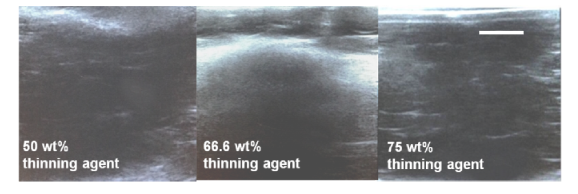
\includegraphics[width=0.8\textwidth]{Рисунки/ПДМС.png}
\caption{\centering Сравнение ультразвуковых изображений фантома с различным содержанием ПДМС}
\label{оболочка}
\end{center}
\end{figure}

\section{Выводы к главе 1}
В ходе проведенного медико-биологического обзора рассмотрены основные методы трекинга внутрисосудистых инструментов на изображениях с ультразвуковых визуализационных систем, проведен обзор существующих материалов для изготовления фантома мягких тканей, определены основные области применения роботизированных ультразвуковых систем, описана модель биологического объекта. По результатам обзора составлен лист постановки задачи, представленный в приложении A.







